\chapter{Tunable Laser with on Chip Controllable Feedback}\label{ch:laser_with_on_chip_feedback}
\section{Design}\label{sec:design}
\begin{figure}[ht]
    \centering
    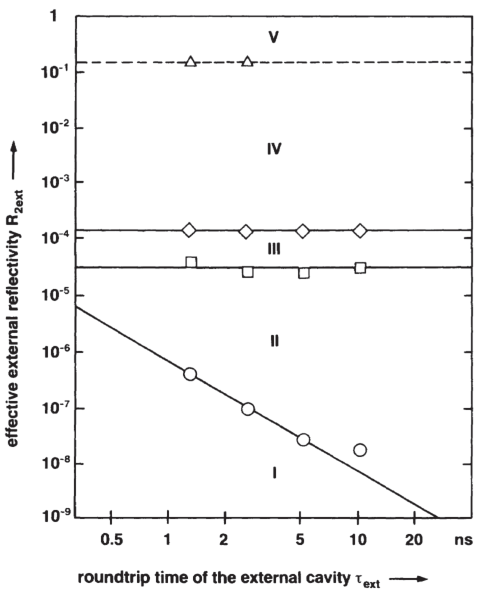
\includegraphics[width=10cm]{figures/feedback_region.PNG}
    \caption{Feedback regimes for a laser diode.}
    \label{feedback_region}
\end{figure}
\subsection{Active and Passive Elements}
As a variable optical attenuator (VOA) a 1x1 thermally tunable Multimode interferometer (MMI) is used (Fig.3.4.c). MMI is a multimode waveguide in which the light propagates in N modes. The various modes interfere with each other and produce an interference pattern in the MMI. This pattern allows at points of constructive interference to place output waveguide and thus to tap multiple outputs, each with a corresponding proportion of the total output power from an input signal. Depending on the design of the structure, the MMI can realize a different power division. On one side along the MMI is placed an electrode that allows using the thermo-optical effect. 
We distinguish the states ON and OFF. In the OFF state, there is no heating of the electrodes and constructive interference takes place at the point where the output waveguide is. In ON-state, the interference pattern of the MMI is so affected, so that shifts through the partial change of the refractive index of the MMI, the position of constructive interference. Thus, a maximum interference point moves away from the position of the output waveguide and the output signal is tapped at reduced power (Fig.3.4.a and b). In this way a variable optical attenuation is created.
An input waveguide with a width and height of 3.2 µm leads light into the interferometer. The height of the MMI (x-axis) also corresponds to 3.2 µm, the width is 18 µm and the length is 380 µm. The light that is leaving the MMI is received by an output waveguide. Height and width of the output waveguide coincide with the dimensions of the input waveguide. The transition of the input and output waveguide of the MMI is realized with taper sections that reduce the coupling losses. This VOA design was showing the best results compare to the literature [16-18].

\subsection{Long Feedback Cavity}

\subsection{Short Feedback Cavity}

\section{Characterization}

\begin{figure}[!htb]
    \centering
    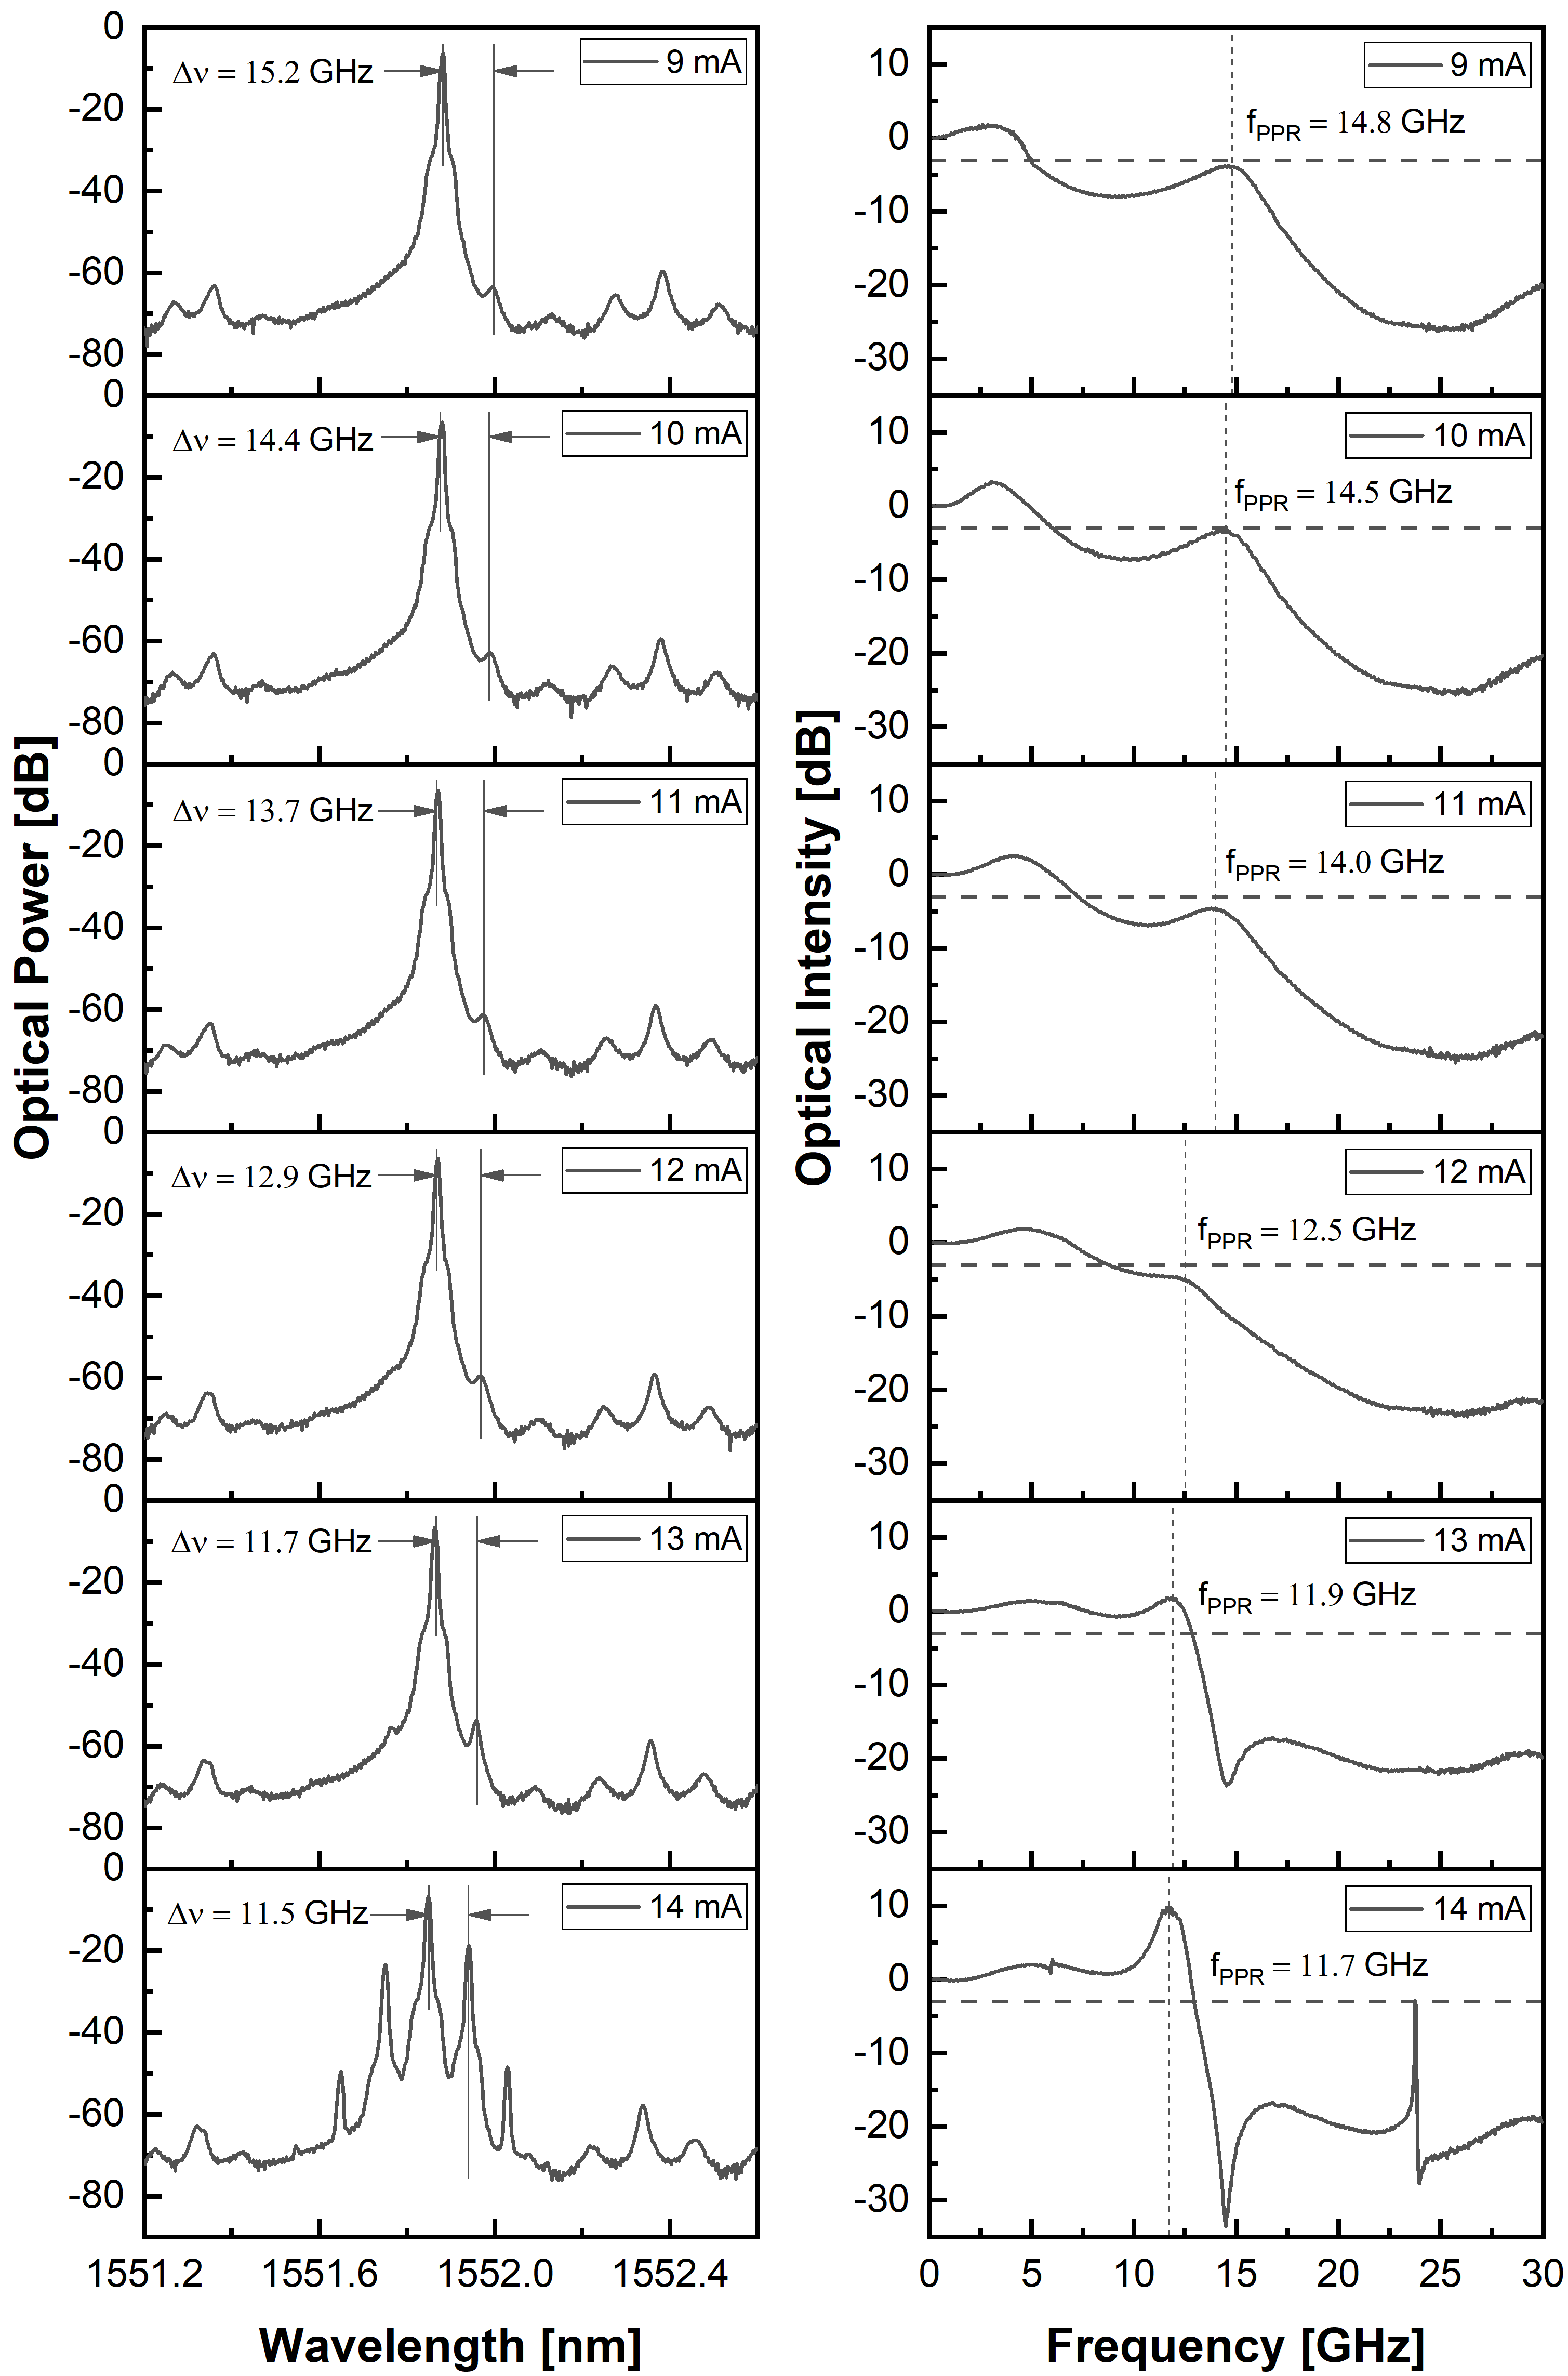
\includegraphics[width=\linewidth]{figures/spectra_and_bandwidth_6559.png}
    \caption{}
    \label{fig:spectra_and_bandwidth_6559}
\end{figure}

\begin{figure}[!htb]
    \centering
    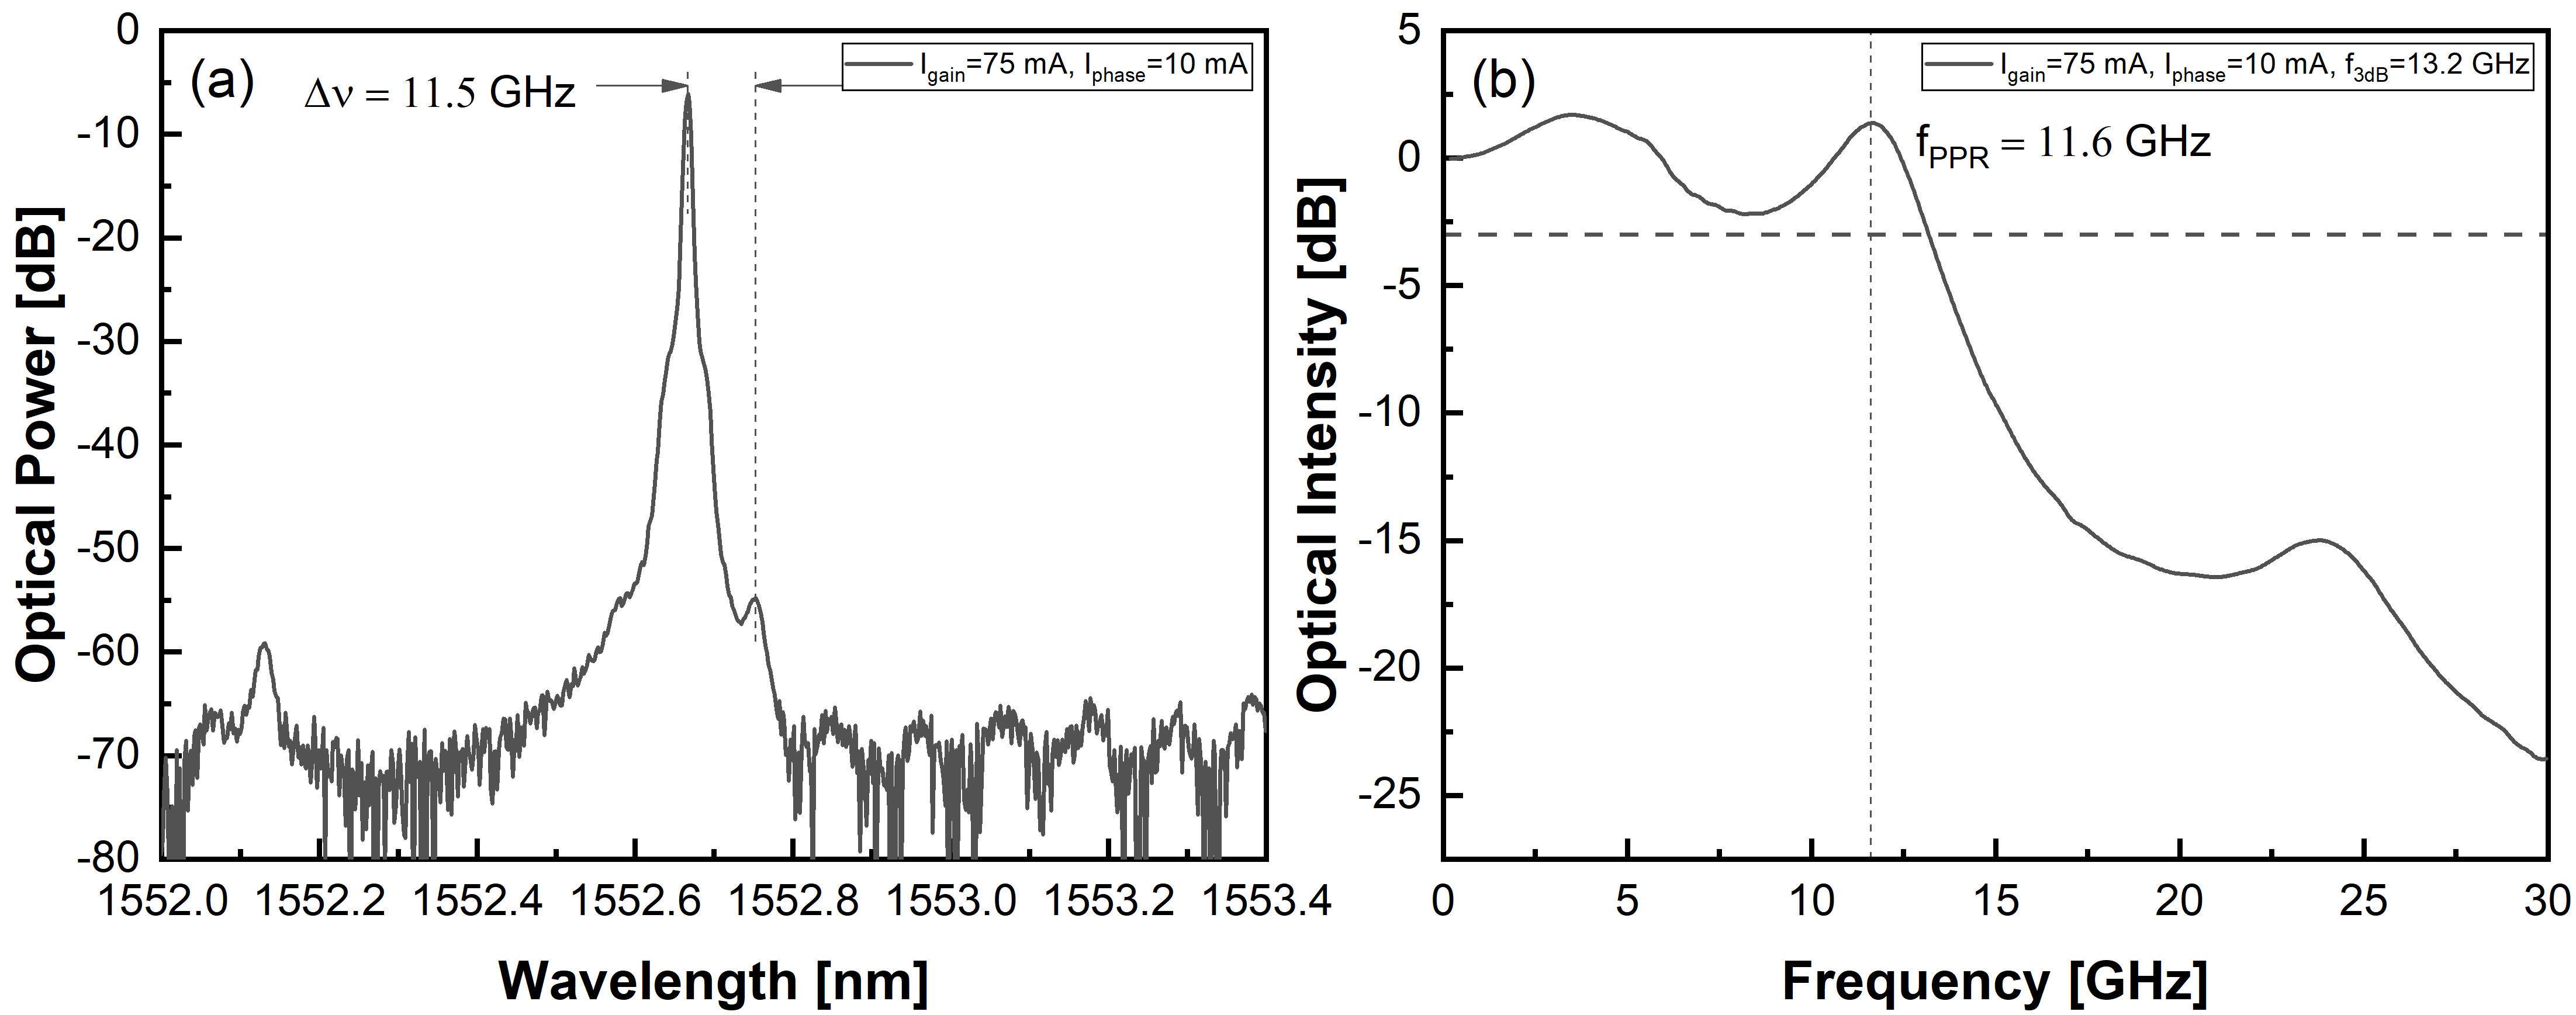
\includegraphics[width=\linewidth]{figures/spectrum_and_bandwidth_6557.png}
    \caption{}
    \label{fig:spectra_and_bandwidth_6557}
\end{figure}

\begin{figure}[!htb]
    \centering
    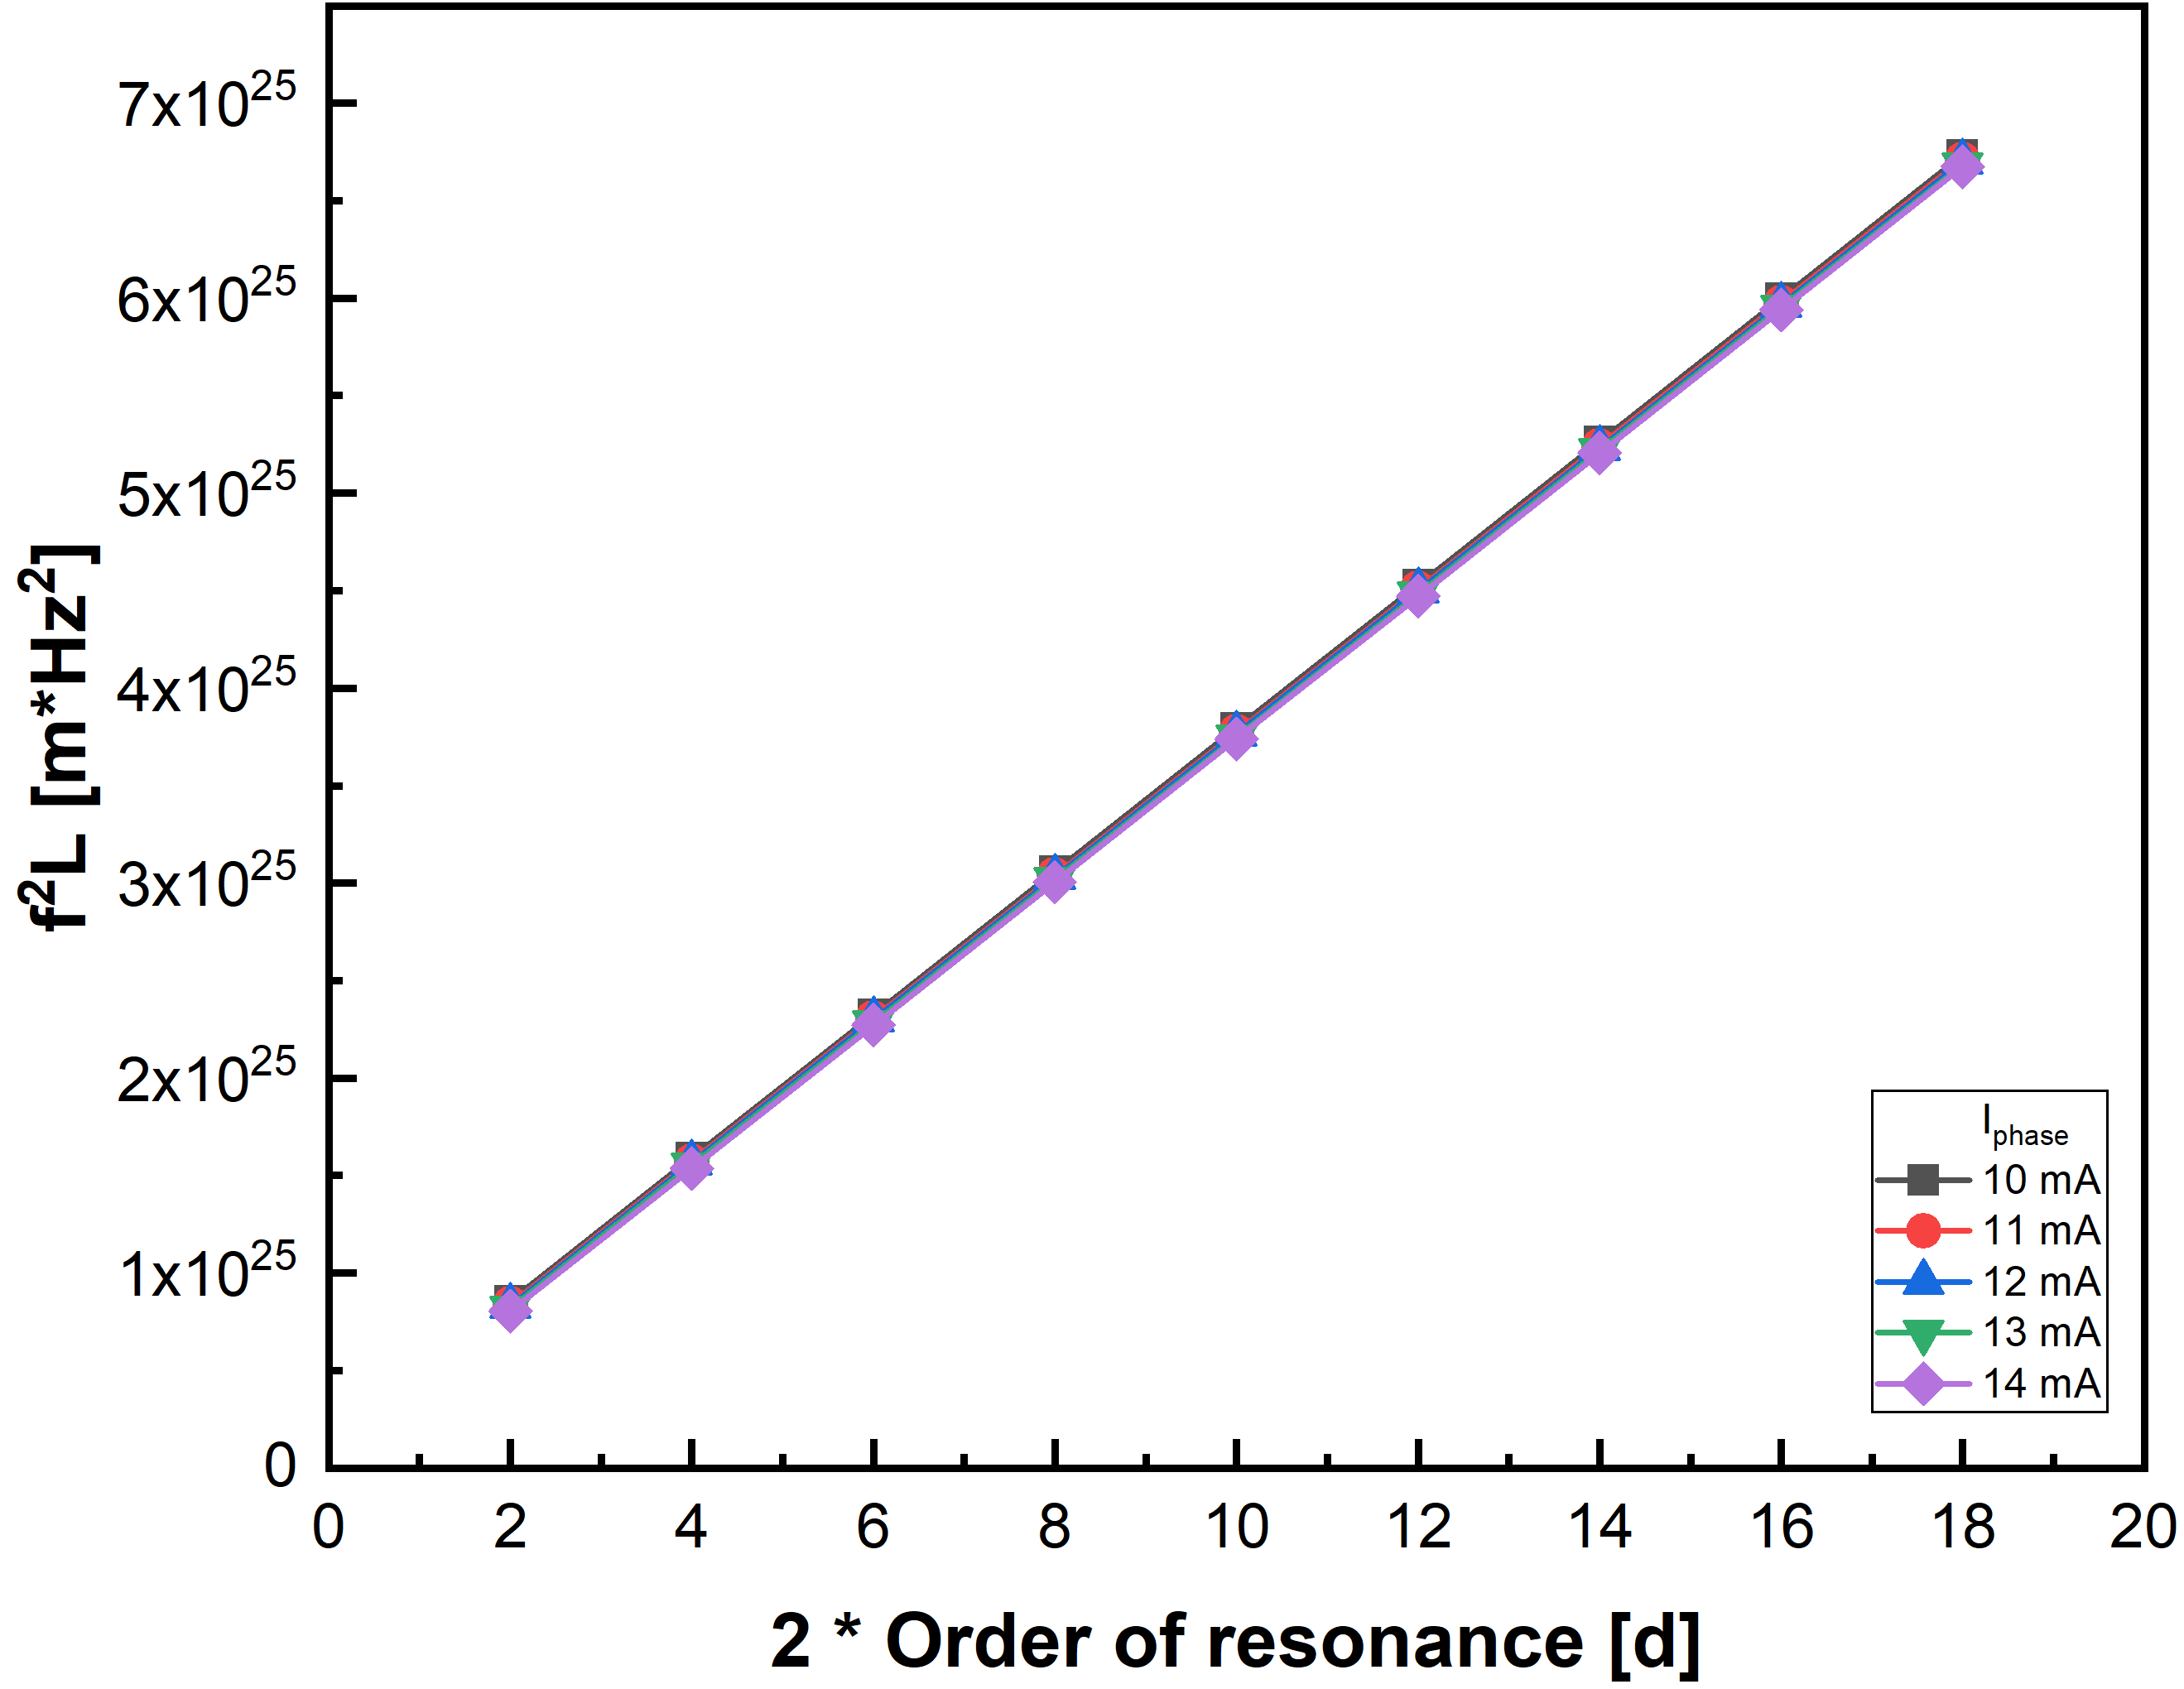
\includegraphics[width=.7\linewidth]{figures/chirp_6559.png}
    \caption{}
    \label{fig:chirp_6559}
\end{figure}

\begin{table}[!htb]
    \centering
    \caption{My caption}
    \label{my-label}
    \begin{tabular}{@{}llllll@{}}
    \toprule
    \multirow{2}{*}{Current {[}mA{]}} & \multicolumn{5}{c}{$\alpha$}                                                                                \\ \cmidrule(l){2-6} 
                                      & $I_{phase}=10 \ mA$ & $I_{phase}=11 \ mA$ & $I_{phase}=12 \ mA$ & $I_{phase}=13 \ mA$ & $I_{phase}=14 \ mA$ \\ \midrule
    75                                & 1.725               & 2.063               & 2.22                & 2.624               & 3.247               \\
    75                                & 1.818               & 1.991               & 2.296               & 2.618               & 3.257               \\
    75                                & 1.818               & 2.07                & 2.246               & 2.614               & 3.253               \\
    75                                & 1.808               & 2.054               & 2.242               & 2.566               & 3.221               \\ \midrule
    Average                           & 1.79225             & 2.0445              & 2.251               & 2.6055              & 3.2445              \\ \bottomrule
    \end{tabular}
\end{table}